\section{Monte-Carlo Simulation} 
Comprehensive Monte-Carlo simulations to check major parameters of the HTCC was done before the design of the detector was completed. Electrons of 2 GeV energy were used.    

\indent On the Fig.\ref{fig:PROPERTIES} are presented MC simulation results of properties of the major components of the detector: transparency of the carbon dioxide radiator gas, reflectivity of mirrors deposited with metal aluminum covered by magnesium fluoride protection coating, and transparency of the PMT entry window material as function of wavelength. As one can see the radiator gas and mirror reveal good optical properties (transmittance and relativity) in the UV-range. As far as the entry window material is concerned, as expected, the quartz window provides the highest signal as opposed to window made of UV-transmitting glass. PMTs with quartz entry windows are significantly more expensive and are also fragile. We have run comparative tests of 5" ET 9823 PMTs with both quartz and UV-transmitting glass windows to justify better solution. 

On the Fig.\ref{fig:Quartz_UV_glass} are shown obtained results. As measurements have shown the average signal from PMT with quartz window is equivalent of 55.6 phe whereas for the PMT with UV-transmitting glass the average signal is only of 38.2 phe. These tests have proven the advantages of a PMT with a quartz window: ~ 45\% more light if we use quartz PMTs.

\begin{figure}[!ht]
    \centering
    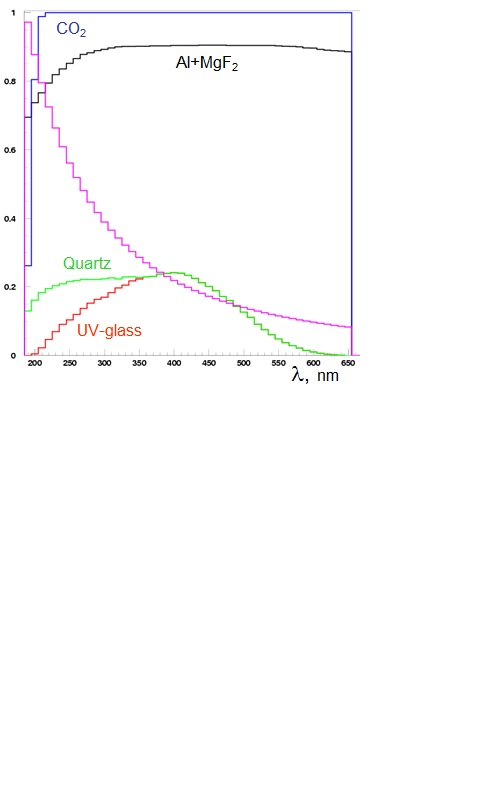
\includegraphics[width=1.0\linewidth,trim={0.0cm 10.7cm 3.7cm 0.1cm},clip]{images/PROPERTIES.jpg}
    \caption{Optical properties of the HTCC major components. Exponential histogram (magenta) describes Cerenkov light spectrum}
    \label{fig:PROPERTIES}
\end{figure}

\begin{figure}[!ht]
    \centering
    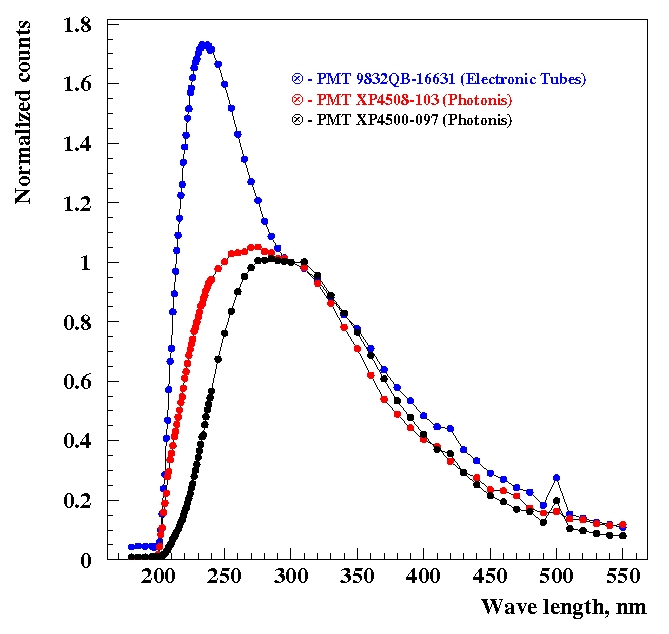
\includegraphics[width=1.0\linewidth,trim={1.7cm 0.5cm 0.05cm 0.1cm},clip]{images/Quartz_UV_glass.jpg}
    \caption{Comparative test results on the transparency of PMT windows made of Quartz (blue), UV-transmitting glass (red) and regular glass (black)}
    \label{fig:Quartz_UV_glass}
\end{figure}

Photomultiplier tubes are available with a face plate (entry window) that can be in various shapes. In the HTCC Cerenkov light is generated along the entire length of a scattered electron's trajectory in the working volume of the detector. The light collection geometry provided by the fully ellipsoidal mirror with point-to-point focusing is valid only in the case when one focal point is in the target position and when the second focal point is at the face of the light detector (PMT). Consequently one must expect considerable changes in the size of image in the focal plane due to the continuous slipping of the light emission point along the electron trajectory. Moreover there is no light emitted by a scattered electron moving from the target until it crosses the entry window of the HTCC and is them detected by the detector. Photomultiplier tubes of large size are available with a face plate (entry window) of various shapes. This is one more parameter to check. A light collection pattern has been simulated for the exact HTCC geometry to answer following basic questions with regards to the detector:

\begin{itemize}
\item Which shape (convex or flat) has the most efficient light collection?
\item What window material has to be used to provide the highest possible signal strength?
\item What are the actual image dimensions in the focal planes?
\item What would be the basic dimensions of a Winston Light Concentrator, if we had to use them?
\end{itemize}

In the Fig.\ref{fig:Flat_Convex} are shown simulation results on the collection of light impinging on the entry window for two different PMTs, comparing those with convex windows and those with flat windows. 

\begin{figure}[!ht]
    \centering
    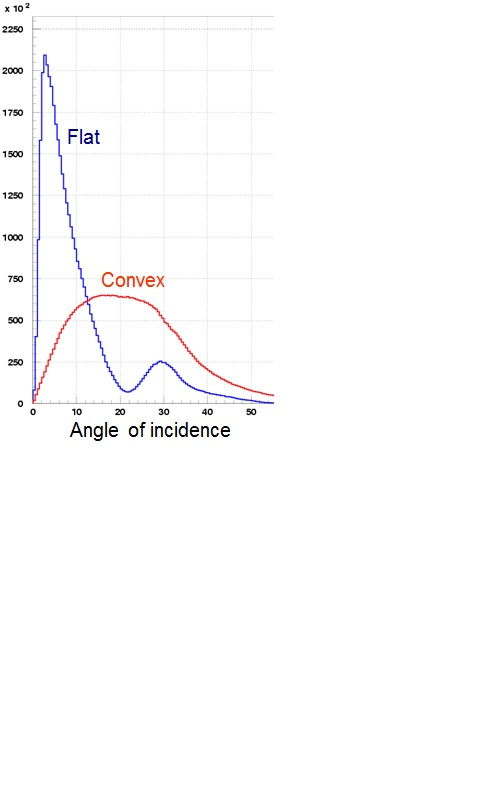
\includegraphics[width=1.0\linewidth,trim={0.0cm 9.1cm 6.3cm 0.1cm},clip]{images/Flat_Convex.jpg}
    \caption{Distribution of Photons impinging on the PMT face plate}
    \label{fig:Flat_Convex}
\end{figure}

Clearly the flat entry window is preferable. From the Fig.\ref{fig:Flat_Convex} we also estimated that about 80\% of Cerenkov light will directly impinging the PMT photocathode and remaining 20\% of light will be reflected by Winston Cone first. The 5" quartz phototube ET-9823QKB used in the HTCC has a photocathode that is actually 110 mm in diameter ($\sim$4.3"). 

In the following pictures Fig.\ref{fig:Point_Targ_Zero_Field_PMT}, Fig.\ref{fig:Point_Targ_5T_Field_PMT}, Fig.\ref{fig:10cm_Targ_5T_Field_PMT} results of the MC simulations of the light collection on the face of PMT1, which is detecting light reflected by a mirror facet that covers a polar angle range of 5$^\circ$ to 12.5$^\circ$ are presented. \\
\indent Data are obtained for 2 GeV electrons for a point-like target without and with 5T solenoidal field generated by the Central Superconductive Solenoid (CSS), and for a 10 cm long target with a 5T field. On all three pictures are shown the white circle (Ø 110 mm) represents the boundary of the PMT light sensitive area. The light collection is not much sensitive on the field of solenoid especially if the target is short. There are only small changes. Data are presented in the logarithmic scale so the most of the light is impinging the photocathode directly. 
In the real experiments with electron beam the 5 cm long cryogenic targets are used. 

Estimates for signal strength for 2 GeV electrons have been obtained also for point-like and extended targets with and without 5T field. \\
\indent Similar simulation results are obtained for patterns on the face of Winston Light Concentrators. On the Fig.\ref{fig:10cm_Targ_5T_Field_WCone} are shown result for 10 cm long target in the 5T field. There is a circle of diameter 161.4 mm shown on the picture just for illustration of possible Winston Cone opening diameter. Based on these results the Winston Light Concentrators used in the HTCC have a fully circular opening of radius R=7.4 cm and length of 190 mm, leaving the PMT photocathode completely open. Reflective surfaces of the mirrors and Winston Cones unavoidably will have certain imperfections and correspondingly will lead to smeared patterns. 

\begin{figure}[!ht]
    \centering
    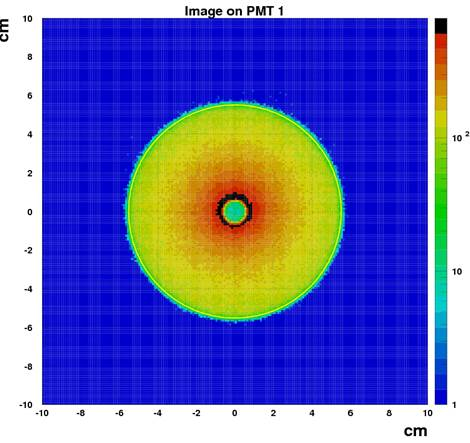
\includegraphics[width=1.0\linewidth,trim={0.0cm 0.0cm 0.0cm 0.0cm},clip]{images/Point_Targ_Zero_Field_PMT.jpg}
    \caption{Light collection pattern on the face of the PMT for point-like target and no solenoidal field}
    \label{fig:Point_Targ_Zero_Field_PMT}
\end{figure}

\begin{figure}[!ht]
    \centering
    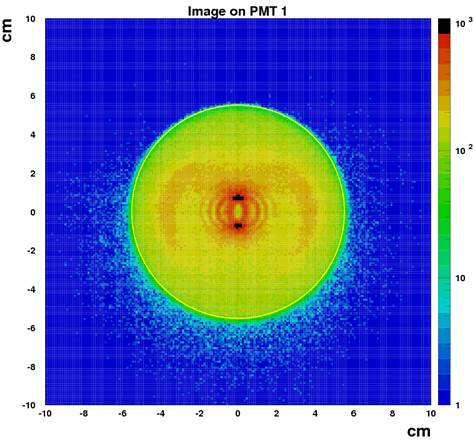
\includegraphics[width=1.0\linewidth,trim={0.0cm 0.0cm 0.0cm 0.0cm},clip]{images/Point_Targ_5T_Field_PMT.jpg}
    \caption{Light collection pattern on the face of the PMT for point-like target and 5T solenoidal field}
    \label{fig:Point_Targ_5T_Field_PMT}
\end{figure}

\begin{figure}[!ht]
    \centering
    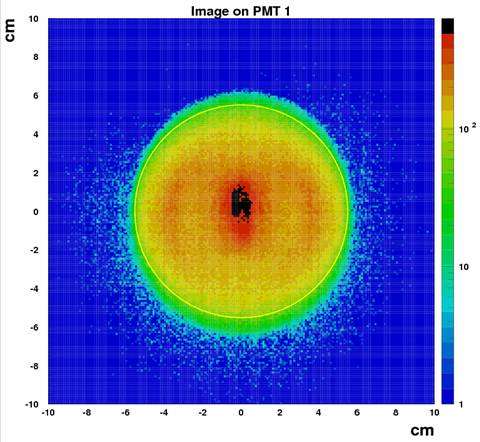
\includegraphics[width=1.0\linewidth,trim={0.0cm 0.0cm 0.0cm 0.0cm},clip]{images/10cm_Targ_5T_Field_PMT.jpg}
    \caption{Light collection pattern on the face of the PMT for point-like target and 5T solenoidal field}
    \label{fig:10cm_Targ_5T_Field_PMT}
\end{figure}

\begin{figure}[!ht]
    \centering
    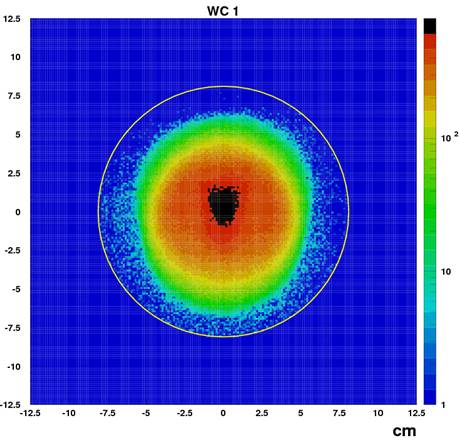
\includegraphics[width=1.0\linewidth,trim={0.0cm 0.0cm 0.0cm 0.0cm},clip]{images/10cm_Targ_5T_Field_WCone.jpg}
    \caption{Light collection pattern on the face of the PMT for point-like target and 5T solenoidal field}
    \label{fig:10cm_Targ_5T_Field_WCone}
\end{figure}

Estimates for signal strength for 2 GeV electrons have been obtained also for the point-like and extended targets with and without 5T field.\\
\indent The following pictures 
Fig.\ref{fig:Point_Targ_Zero_Field_Theta}, 
Fig.\ref{fig:Point_Targ_5T_Field_Theta}, and 
Fig.\ref{fig:10cm_Targ_5T_Field_Theta} 
present angular distributions in the the polar angle range. Histograms  in the the azimuthal angle range are shown on the 
Fig.\ref{fig:Point_Targ_Zero_Field_Phi}, 
Fig.\ref{fig:Point_Targ_5T_Field_Phi}, and 
Fig.\ref{fig:10cm_Targ_5T_Field_Phi}. 

\begin{figure}[!ht]
    \centering
    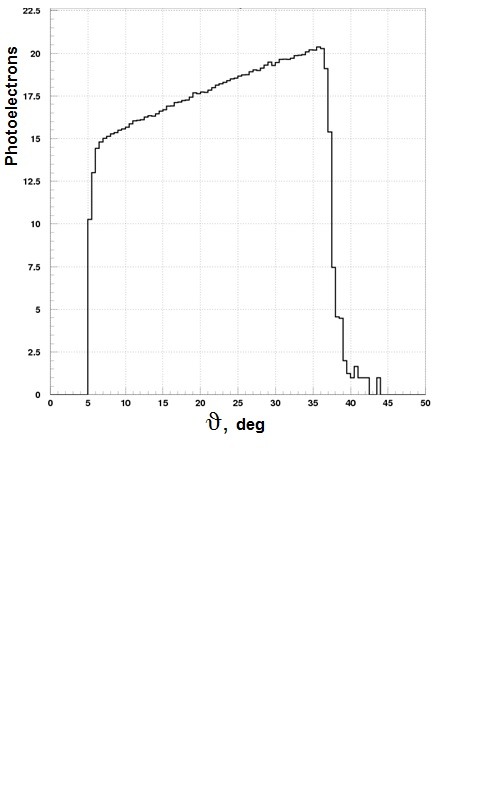
\includegraphics[width=1.0\linewidth,trim={0.0cm 9.4cm 0.0cm 0.0cm},clip]{images/Point_Targ_Zero_Field_Theta.jpg}
    \caption{Signal strength as function of polar angle. Point-like target and no solenoidal field}
    \label{fig:Point_Targ_Zero_Field_Theta}
\end{figure}

\begin{figure}[!ht]
    \centering
    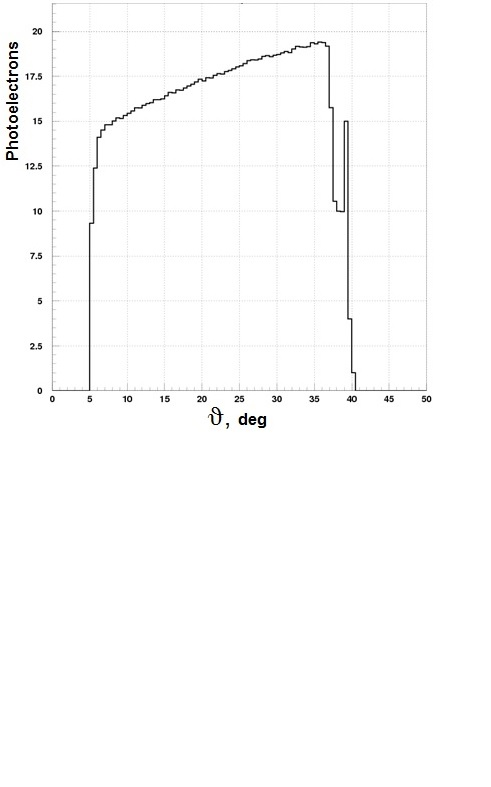
\includegraphics[width=1.0\linewidth,trim={0.0cm 9.4cm 0.0cm 0.0cm},clip]{images/Point_Targ_5T_Field_Theta.jpg}
    \caption{Signal strength as function of polar angle. Point-like target and 5T solenoidal field}
    \label{fig:Point_Targ_5T_Field_Theta}
\end{figure}

\begin{figure}[!ht]
    \centering
    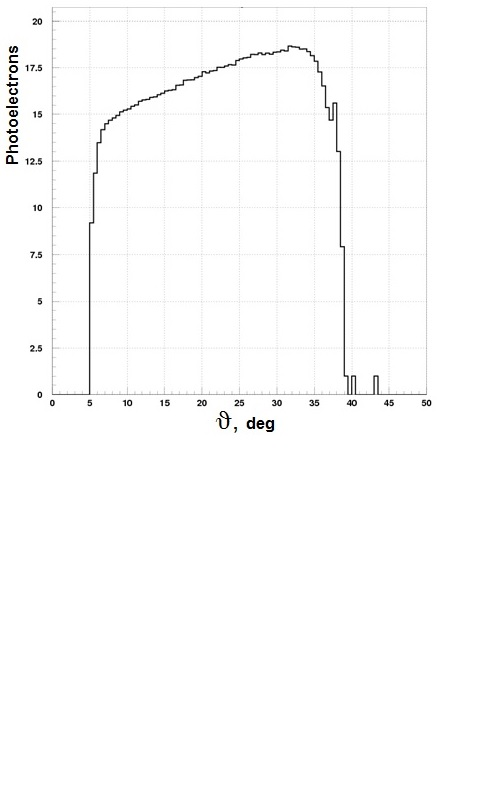
\includegraphics[width=1.0\linewidth,trim={0.0cm 9.4cm 0.0cm 0.0cm},clip]{images/10cm_Targ_5T_Field_Theta.jpg}
    \caption{Signal strength as function of polar angle. 10cm long target and 5T solenoidal field}
    \label{fig:10cm_Targ_5T_Field_Theta}
\end{figure}

One can see that the signal strength is increasing with the polar angle. This is because the electrons scattered at a smaller angle travel a shorter distance in the radiator gas as compared to the electrons moving under larger angles. The minimum signal strength is estimated to be about 14–15 photoelectrons (phe). For electrons scattered in range of polar angles from $5^\circ$ to $35^\circ$
we have a complete and uniform coverage of entire 2$\pi$ acceptance, as demonstrated by the azimuthal dependencies. The average signal strength is about 17 phe. This estimate have been obtained by taking into consideration possible reduction of mirror reflectivity due to the unavoidable degradation of the reflective surface during the construction stage (limited stability of reflectivity, dust and fume deposition, mechanical defects etc.) that has first been observed after the construction of the Low Threshold Cerenkov Counter for the CLAS spectrometer.

\begin{figure}[!ht]
    \centering
    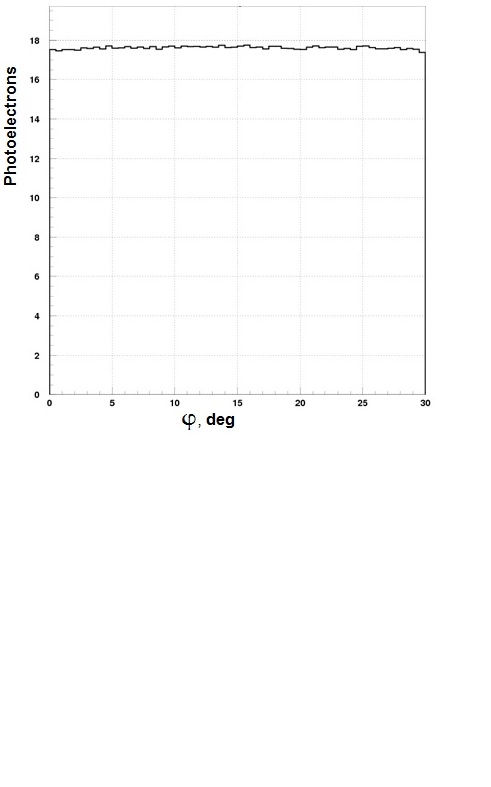
\includegraphics[width=1.0\linewidth,trim={0.0cm 9.4cm 0.0cm 0.0cm},clip]{images/Point_Targ_Zero_Field_Phi.jpg}
    \caption{Signal strength as function of polar angle. Point-like target and no solenoidal field}
    \label{fig:Point_Targ_Zero_Field_Phi}
\end{figure}

\begin{figure}[!ht]
    \centering
    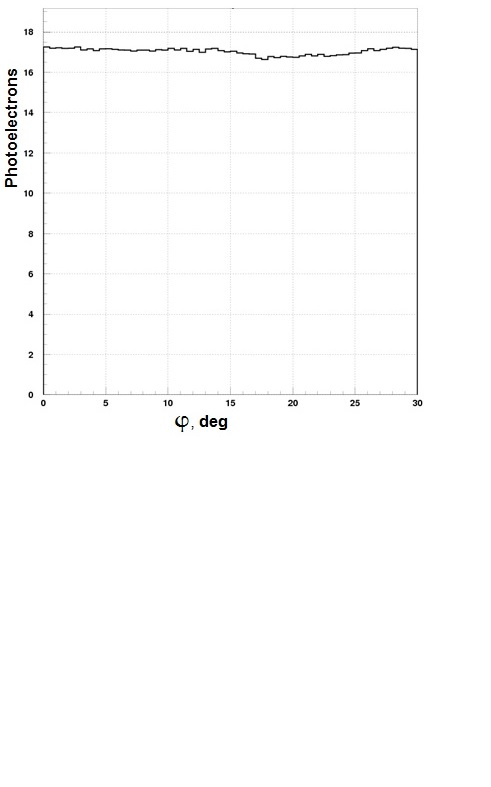
\includegraphics[width=1.0\linewidth,trim={0.0cm 9.4cm 0.0cm 0.0cm},clip]{images/Point_Targ_5T_Field_Phi.jpg}
    \caption{Signal strength as function of polar angle. Point-like target and 5T solenoidal field}
    \label{fig:Point_Targ_5T_Field_Phi}
\end{figure}

\begin{figure}[!ht]
    \centering
    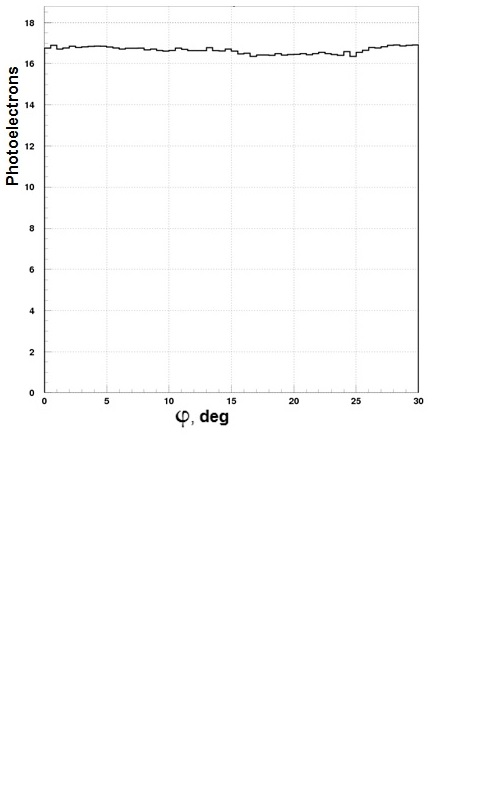
\includegraphics[width=1.0\linewidth,trim={0.0cm 9.4cm 0.0cm 0.0cm},clip]{images/10cm_Targ_5T_Field_Phi.jpg}
    \caption{Signal strength as function of polar angle. 10cm long target and 5T solenoidal field}
    \label{fig:10cm_Targ_5T_Field_Phi}
\end{figure}

\indent One of sources of background events in the HTCC are the secondary interactions of charged pions with components in the working volume of the HTCC and as with components outside the detector in the region between the target and the entry window. Charged pions with energies mostly bellow the detection threshold can knock out relativistic $\delta$ -electrons that generate Cerenkov light in the working volume. Some of that light can be focused by the mirror on the photomultiplier tubes. In our MC simulations we estimated expected background rates. Of course rates depend on actual amount and distribution of materials. We have specified in details  everything regarding the detector components. With regard outside components we have taken into account the 10 cm long cryogenic target filled with hydrogen, standard scattering chamber and air gap between exit window of the chamber and entry window of the HTCC. \\
\indent At the CLAS12 designed luminosity of L $\approx$ 10$^{35}$ cm$^{-2}$ sec$^{-1}$ the estimated of total background rate for one half-sector is about 20 kHz. \\  
\indent The most important parameters for the Cerenkov counters are the electron detection efficiency and the charged pion rejection power. In the Fig.\ref{fig:Pion_rejection_2GeV} simulation results on rejection of charged pions are shown. Data are presented for four HTCC channels from one half-sector at three different thresholds of electron detection at 2 GeV: equivalent of 1, 2 and 3 photoelectrons. 

\begin{figure}[!ht]
    \centering
    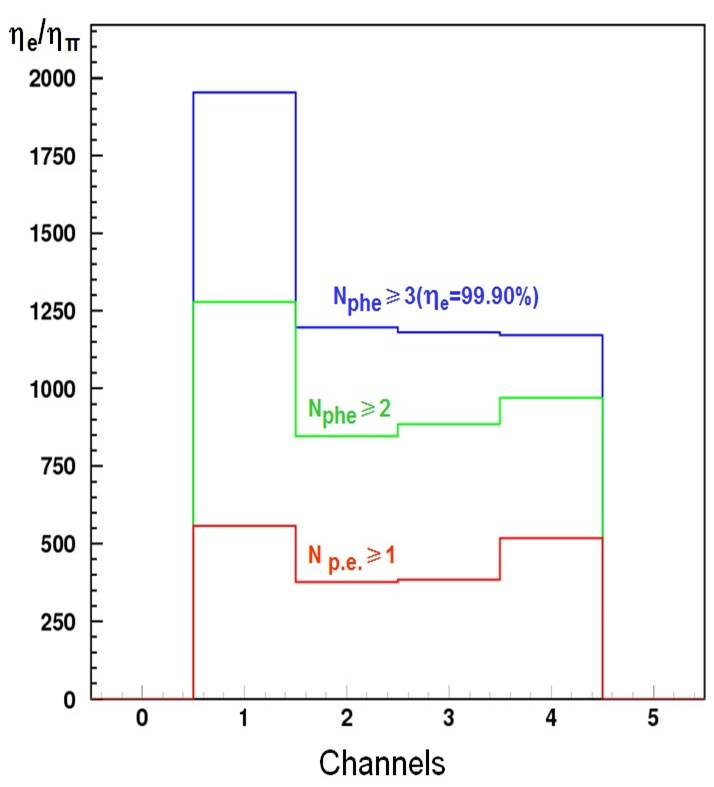
\includegraphics[width=1.0\linewidth,trim={0.0cm 0.0cm 0.0cm 0.0cm},clip]{images/Pion_rejection_2GeV.jpg}
    \caption{Rejection of charged pions at 2 GeV}
    \label{fig:Pion_rejection_2GeV}
\end{figure}

For the highest electron detection threshold there is given a corresponding estimate for the electron detection efficiency. At lower thresholds efficiencies are close to 100\%. \\
\indent Similar results for the 4 GeV electrons at shown in the Fig.\ref{fig:Pion_rejection_4GeV}. 

\begin{figure}[!ht]
    \centering
    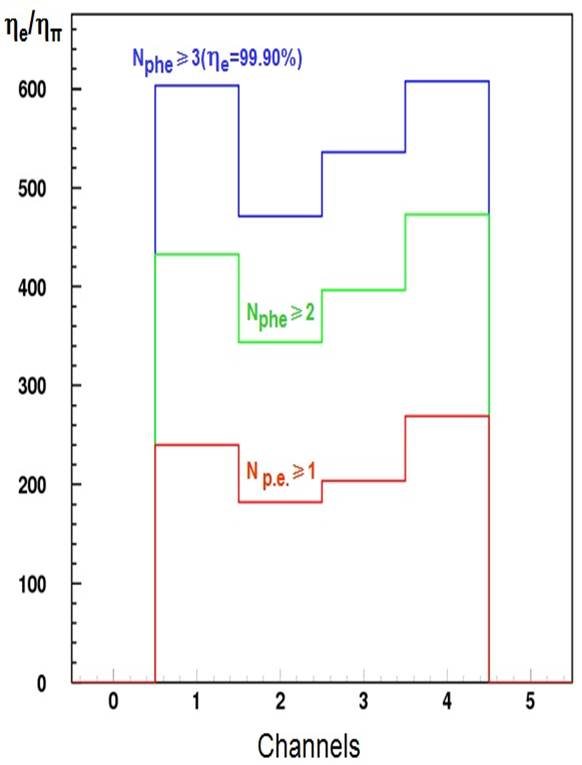
\includegraphics[width=1.0\linewidth,trim={0.0cm 0.0cm 0.0cm 0.0cm},clip]{images/Pion_rejection_4GeV.jpg}
    \caption{Rejection of charged pions at 4 GeV}
    \label{fig:Pion_rejection_4GeV}
\end{figure}

One can conclude that at the threshold of 3 phe the average rejection factor is greater than 1000 at 2 GeV and at least 500 at 4 GeV. At the same time electron detection efficiency is close to 100\%.
